\documentclass[11pt]{article}
\usepackage[utf8]{inputenc}
\usepackage[T1]{fontenc}
\usepackage{amsmath}
\usepackage{multicol}
\usepackage{geometry}
\usepackage{tikz}
\usetikzlibrary{shapes.geometric, arrows.meta}
\usepackage{enumitem}
\usepackage{xcolor}
\usepackage{titlesec}
\usepackage{parskip}
\setlength{\parskip}{0.5em}
\renewcommand{\baselinestretch}{1.0}

% Configurações de layout
\geometry{a4paper, left=1cm, right=1cm, top=0.5cm, bottom=1.2cm}
\setlength{\columnseprule}{0.4pt}
\setlength{\baselineskip}{1.0\baselineskip}

% Cores para títulos
\titleformat{\section}{\normalfont\Large\bfseries\color{blue}}{\thesection}{1em}{}
\titleformat{\subsection}{\normalfont\large\bfseries\color{red}}{\thesubsection}{1em}{}
\titleformat{\subsubsection}{\normalfont\normalsize\bfseries\color{black}}{\thesubsubsection}{1em}{}

\title{\textcolor{blue}{Função Logarítmica: Definição e Aplicações}}
\author{Professor: Jefferson}
\date{}

\begin{document}

\maketitle
\vspace{-1cm}

\begin{center}
    \large{Nome: \underline{\hspace{8cm}} \quad Turma: \underline{\hspace{3cm}}}
\end{center}

\begin{multicols}{2}

    \section*{1. Definição}
    A função logarítmica é a inversa da função exponencial:
    \[
        y = \log_b x \quad \Leftrightarrow \quad b^y = x
    \]
    onde:
    \begin{itemize}
        \item $b$ é a base ($b > 0$, $b \neq 1$)
        \item $x$ é o logaritmando ($x > 0$)
        \item $y$ é o logaritmo
    \end{itemize}

    \subsection*{Exemplos Característicos}
    \begin{itemize}
        \item Logaritmo decimal: $f(x) = \log_{10} x$ ou $\log x$
        \item Logaritmo natural: $g(x) = \ln x$ (base $e \approx 2,718$)
        \item Com base 2: $h(x) = \log_2 x$
        \item Com deslocamento: $p(x) = \log_3 (x + 2)$
    \end{itemize}

    \section*{2. Propriedades Fundamentais}
    Para $a, b > 0$, $b \neq 1$, $x, y > 0$:
    
    \begin{enumerate}
        \item $\log_b (x \cdot y) = \log_b x + \log_b y$
        \item $\log_b \left(\frac{x}{y}\right) = \log_b x - \log_b y$
        \item $\log_b (x^p) = p \cdot \log_b x$
        \item $\log_b b = 1$
        \item $\log_b 1 = 0$
        \item Mudança de base: $\log_a x = \frac{\log_b x}{\log_b a}$
    \end{enumerate}

    \section*{3. Gráficos e Comportamento}
    
    \begin{center}
    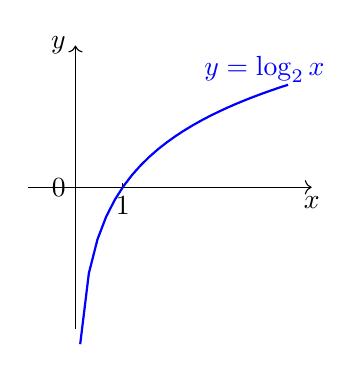
\begin{tikzpicture}[scale=0.6]
        % Eixos
        \draw[->] (-1,0) -- (5,0) node[below] {$x$};
        \draw[->] (0,-3) -- (0,3) node[left] {$y$};
        \draw[thick, blue, domain=0.1:4.5] plot (\x, {ln(\x)/ln(2)});
        \node[blue] at (4,2.5) {$y = \log_2 x$};
        \draw[dashed] (1,0) -- (1,0.1);
        \node[below] at (1,0) {1};
        \draw[dashed] (0,0) -- (0.1,0);
        \node[left] at (0,0) {0};
    \end{tikzpicture}
    \end{center}

    \textbf{Características:}
    \begin{itemize}
        \item Domínio: $(0, +\infty)$
        \item Imagem: $\mathbb{R}$
        \item Contínua e injetora
        \item Crescente se $b > 1$
        \item Decrescente se $0 < b < 1$
        \item Assíntota vertical: $x = 0$
    \end{itemize}

    \section*{4. Exercícios Básicos}
    
    \begin{enumerate}
        \item Calcule os logaritmos:
        \begin{enumerate}[label=\alph*)]
            \item $\log_2 8$
            \item $\log_{10} 1000$
            \item $\log_3 \frac{1}{9}$
            \item $\ln e^5$
        \end{enumerate}
        
        \item Resolva as equações:
        \begin{enumerate}[label=\alph*)]
            \item $\log_3 x = 4$
            \item $\log_5 (2x - 1) = 2$
            \item $\log_2 (x^2 - 3) = \log_2 6$
        \end{enumerate}
        
        \item Aplique as propriedades:
        \begin{enumerate}[label=\alph*)]
            \item $\log_2 (8 \times 16)$
            \item $\log_3 \frac{27}{9}$
            \item $\log_5 25^3$
        \end{enumerate}
        
        \item Simplifique as expressões:
        \begin{enumerate}[label=\alph*)]
            \item $\log_2 8 + \log_2 4 - \log_2 2$
            \item $2\log_3 9 - 3\log_3 3$
            \item $\frac{\log_5 125}{\log_5 25}$
        \end{enumerate}
    \end{enumerate}

    \section*{5. Mudança de Base}
    
    \[
    \log_a b = \frac{\log_c b}{\log_c a}
    \]
    
    \begin{enumerate}
        \item Use mudança de base para calcular:
        \begin{enumerate}[label=\alph*)]
            \item $\log_3 7$ (use base 10)
            \item $\log_5 2$ (use base $e$)
            \item $\log_2 5$ (use base 10)
        \end{enumerate}
        
        \item Prove que: $\log_a b \cdot \log_b a = 1$
        
        \item Calcule: $\log_4 8$ (dica: escreva como potências de 2)
    \end{enumerate}

    \columnbreak
    
    \section*{6. Aplicações Práticas}
    
    \subsection*{1. Escalas Logarítmicas}
    \begin{itemize}
        \item \textbf{Escala Richter} (terremotos):
        \[
        M = \log_{10} \left(\frac{A}{A_0}\right)
        \]
        onde $A$ é a amplitude medida e $A_0$ é amplitude de referência.
        
        \begin{enumerate}[label=\alph*)]
            \item Um terremoto tem amplitude $10^6$ vezes maior que $A_0$. Qual sua magnitude?
            \item Quantas vezes um terremoto de magnitude 7 é mais intenso que um de magnitude 5?
        \end{enumerate}
        
        \item \textbf{Escala Decibel} (som):
        \[
        dB = 10 \cdot \log_{10} \left(\frac{I}{I_0}\right)
        \]
        onde $I$ é a intensidade sonora e $I_0$ é o limiar da audição.
        
        \begin{enumerate}[label=\alph*)]
            \item Um som tem intensidade $10^8$ vezes maior que $I_0$. Quantos decibéis?
            \item Um som de 60 dB é quantas vezes mais intenso que um de 30 dB?
        \end{enumerate}
    \end{itemize}
    
    \subsection*{2. Química - pH de Soluções}
    \[
    pH = -\log_{10} [H^+]
    \]
    onde $[H^+]$ é a concentração de íons hidrogênio (mol/L).
    
    \begin{enumerate}[label=\alph*)]
        \item Calcule o pH de uma solução com $[H^+] = 10^{-3}$ mol/L
        \item Qual a concentração de $H^+$ em uma solução com pH = 5?
        \item Quantas vezes uma solução de pH 3 é mais ácida que uma de pH 6?
    \end{enumerate}
    
    \subsection*{3. Matemática Financeira}
    \begin{itemize}
        \item \textbf{Tempo para atingir um montante} com juros compostos:
        \[
        t = \frac{\log\left(\frac{M}{C}\right)}{\log(1 + i)}
        \]
        onde $M$ é montante, $C$ capital, $i$ taxa.
        
        \begin{enumerate}[label=\alph*)]
            \item R\$ 1000 aplicados a 5\% ao ano. Quando atingirá R\$ 2000?
            \item Em quanto tempo um capital dobra a 10\% ao ano?
        \end{enumerate}
        
        \item \textbf{Depreciação}:
        \[
        t = \frac{\log\left(\frac{V}{V_0}\right)}{\log(1 - d)}
        \]
        onde $V_0$ valor inicial, $V$ valor final, $d$ taxa de depreciação.
        
        \begin{enumerate}[label=\alph*)]
            \item Um carro de R\$ 40.000 deprecia 15\% ao ano. Quando valerá R\$ 20.000?
        \end{enumerate}
    \end{itemize}
    
    \subsection*{4. Biologia - Crescimento Populacional}
    \[
    t = \frac{\log\left(\frac{P}{P_0}\right)}{\log(1 + r)}
    \]
    onde $P_0$ população inicial, $P$ população final, $r$ taxa de crescimento.
    
    \begin{enumerate}[label=\alph*)]
        \item Uma população de 1000 bactérias cresce 20\% por hora. Quando atingirá 5000?
        \item Uma cidade tem 50.000 habitantes e cresce 3\% ao ano. Quando terá 100.000?
    \end{enumerate}
    
    \subsection*{5. Geologia - Datação por Carbono-14}
    \[
    t = \frac{\ln\left(\frac{A}{A_0}\right)}{-k}
    \]
    onde $A_0$ atividade inicial, $A$ atividade atual, $k$ constante de decaimento.
    
    \begin{enumerate}[label=\alph*)]
        \item Um fóssil tem 25\% do C-14 original. Qual sua idade? ($k \approx 0,000121$ ano$^{-1}$)
        \item Se a meia-vida do C-14 é 5730 anos, verifique usando logaritmos.
    \end{enumerate}
    
    \section*{7. Exercícios Avançados}
    
    \begin{enumerate}
        \item Resolva as equações logarítmicas:
        \begin{enumerate}[label=\alph*)]
            \item $\log_2 (x + 3) + \log_2 (x - 3) = 4$
            \item $\log_3 (x^2 - 5x + 7) = 1$
            \item $\log(x - 1) + \log(x + 1) = \log 8$
        \end{enumerate}
        
        \item Sistemas de equações:
        \begin{enumerate}[label=\alph*)]
            \item 
            $\begin{cases}
            \log_2 x + \log_2 y = 5 \\
            x - y = 12
            \end{cases}$
            
            \item
            $\begin{cases}
            \log x + \log y = 2 \\
            xy = 100
            \end{cases}$
        \end{enumerate}
        
        \item Inequações logarítmicas:
        \begin{enumerate}[label=\alph*)]
            \item $\log_2 (x - 1) < 3$
            \item $\log_{\frac{1}{2}} (2x + 4) \geq -2$
            \item $\ln(x^2 - 4) > 0$
        \end{enumerate}
        
        \item Funções compostas:
        \begin{enumerate}[label=\alph*)]
            \item Se $f(x) = \log_2 x$ e $g(x) = 2^x$, calcule $f(g(3))$ e $g(f(8))$
            \item Verifique que $f$ e $g$ são inversas
        \end{enumerate}
        
        \item Problema de otimização:
        \begin{enumerate}[label=\alph*)]
            \item Encontre o domínio da função $f(x) = \log(x^2 - 4x + 3)$
            \item Determine os valores de $x$ para que $\log_3 (x^2 - 1)$ exista
        \end{enumerate}
    \end{enumerate}
    
    \section*{8. Dicas Importantes}
    
    \begin{itemize}
        \item Sempre verifique as condições de existência: logaritmando $> 0$, base $> 0$ e $\neq 1$
        \item Use as propriedades para simplificar expressões
        \item Em equações: $\log_b f(x) = \log_b g(x) \Rightarrow f(x) = g(x)$ (se $f(x), g(x) > 0$)
        \item Em mudança de base, escolha a base mais conveniente (10 ou $e$)
        \item Gráficos: assíntota vertical em $x = 0$, passa por $(1, 0)$
        \item Logaritmo natural ($\ln$) aparece em crescimento/decrescimento contínuo
    \end{itemize}
    
    \section*{9. Resumo das Fórmulas}
    
    \begin{itemize}
        \item $\log_b (xy) = \log_b x + \log_b y$
        \item $\log_b \left(\frac{x}{y}\right) = \log_b x - \log_b y$
        \item $\log_b (x^p) = p \log_b x$
        \item $\log_b b = 1$, $\log_b 1 = 0$
        \item $\log_a b = \frac{\log_c b}{\log_c a}$
        \item $b^{\log_b x} = x$
        \item $\log_b a \cdot \log_a b = 1$
    \end{itemize}

\end{multicols}

\end{document}
